\section{Durchführung}
\label{sec:durchfuehrung}
\subsection{Versuchsaufbau}
Der Versuch wurde mit der Apparatur aus der Abbildung durchgeführt. Es wurde ein Echoskop mit einer $2MHz$ Ultraschallsonde für das Impuls-Echo-Verfahren verwendet.
Die Datenaufnahme erfolgte auf einem Computer mithilfe des Programmes A-Scan. Die Ausmessung des Probenkörpers erfolgte mithilfe einer Schieblehre. Als Kontaktmittel wurden bidestiliertes Wasser sowie Kontaktgel verwendet.
\subsection{Versuchsdurchführung}
Zunächst wurden die Gesamtmaße sowie Tiefe und Durchmesser der Fehlstellen (Löcher) des quaderförmigen Probekörpers mit einer Schieblehre bestimmt.
Anschließend wurde der Probekörper mit der $2Mhz$ Sonde unter Anwendung des Impuls-Echo-Verfahrens untersucht, wobei die den Fehlstellen zugehörigen Laufzeiten $t$ des Signals, sowie der Spannungswert der entsprechenden Amplitude gemessen wurden. Beide lassen sich einfach mithilfe der Cursor aus dem A-Scan Bild ablesen.
Anschließend wurde das Augenmodell, ebenfalls mit der $2Mhz$ Sonde unter Anwendung des Impuls-Echo-Verfahrens, vermessen, um in diesem die Retina zu lokalisieren.

  \begin{figure}[h]
    \label{fig:block}
    \centering
    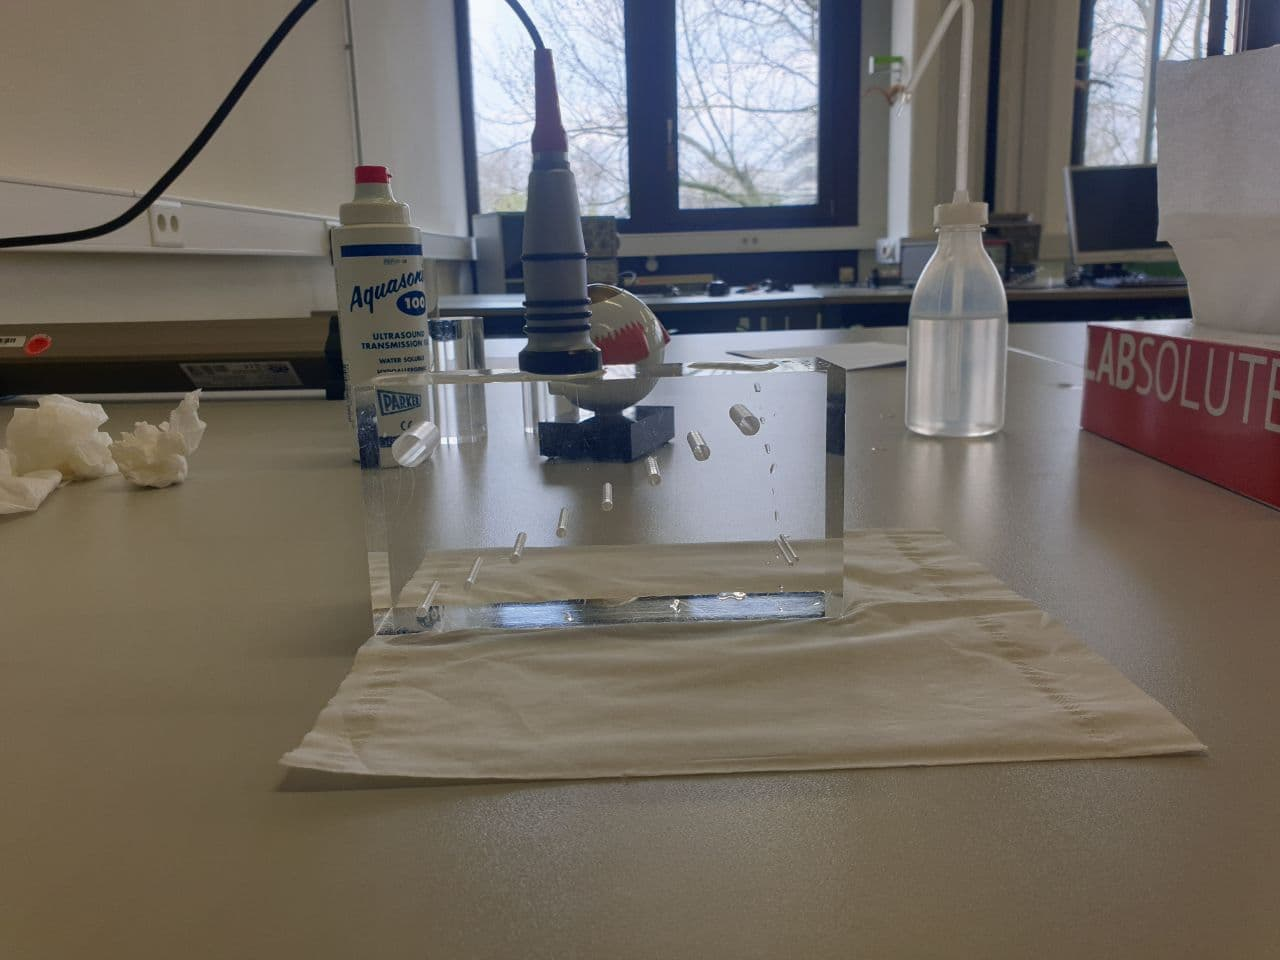
\includegraphics[width=10cm]{Block}
    \caption{Acrylglasblock mit 2-MHz Ultraschall-Sender/Empfänger}
\end{figure}


  \begin{figure}[h]
    \label{fig:aufbau}
    \centering
    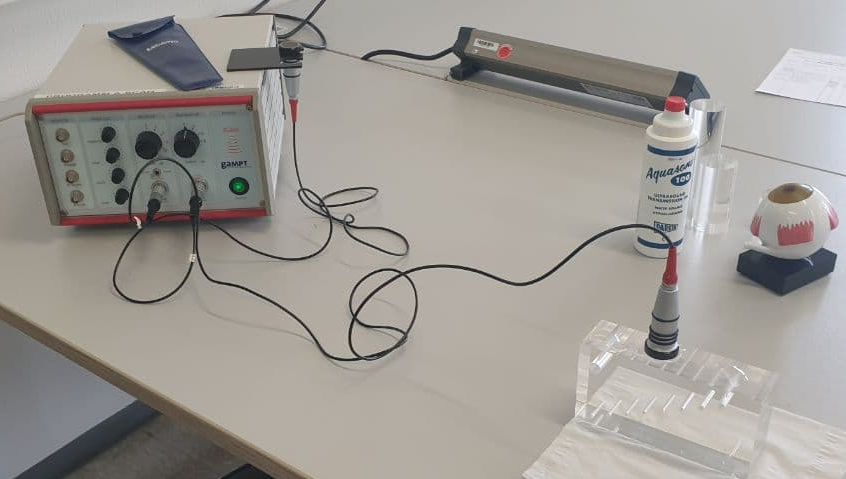
\includegraphics[width=10cm]{Aufbau}
    \caption{Gesamter Versuchsaufbau mit Ultraschallerzeuger. Ultraschall-Sender/-Empfänger, Acrylglasblock und Augenmodell}
\end{figure}
